\begin{center}
Problema C

Revestimento da Piscina

{\tiny Por Márcio Belo-Filho}

Timelimit: $1$	
\end{center}			
			
O professor Márcio pretende fazer uma piscina na sua casa. A piscina é retangular e suas paredes e fundo serão revestidos com azulejos quadrados. Ao final do revestimento alguns azulejos estarão completos e outros estarão cortados, sendo sempre utilizado uma das partes cortadas e outra parte descartada. O professor Márcio quer saber quantos azulejos serão utilizados na piscina e a área total descartada (medida em azulejos). 

A figura abaixo apresenta um exemplo de uma dos lados da piscina, de $5,4$ metros de comprimento por $1,4$ metros de altura, com azulejos de 1 metro de lado. 

\begin{center}
    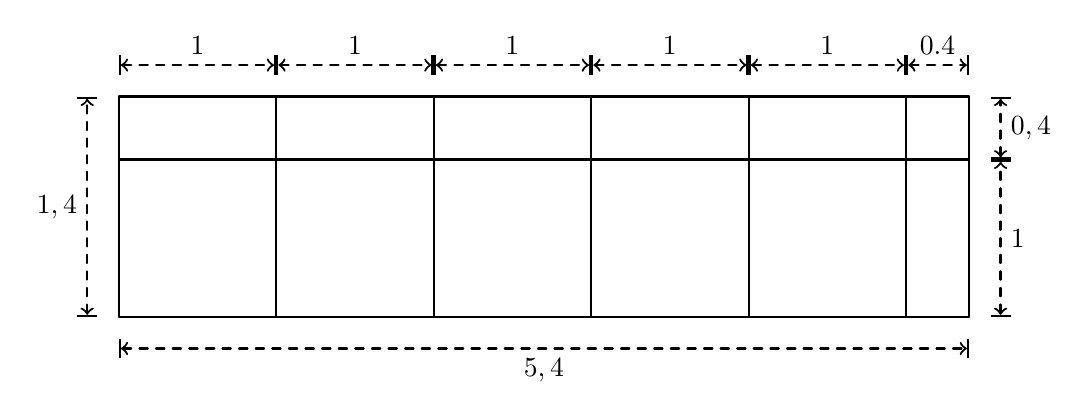
\begin{tikzpicture}[scale=2, line cap=round,line join=round,x=1cm,y=1cm]
        \draw[thick]   (0,0) -- (5.4,0) -- (5.4,1.4) -- (0,1.4) -- cycle; 
        \draw[thick]   (0,0) -- (1,0) -- (1,1) -- (0,1) -- cycle; 
        \draw[thick]   (1,0) -- (2,0) -- (2,1) -- (1,1) -- cycle; 
        \draw[thick]   (2,0) -- (3,0) -- (3,1) -- (2,1) -- cycle;
        \draw[thick]   (3,0) -- (4,0) -- (4,1) -- (3,1) -- cycle;
        \draw[thick]   (4,0) -- (5,0) -- (5,1) -- (4,1) -- cycle;
        \draw[thick]   (5,0) -- (5.4,0) -- (5.4,1) -- (5,1) -- cycle;
        \draw[thick]   (0,1.4) -- (1,1.4) -- (1,1) -- (0,1) -- cycle; 
        \draw[thick]   (1,1.4) -- (2,1.4) -- (2,1) -- (1,1) -- cycle; 
        \draw[thick]   (2,1.4) -- (3,1.4) -- (3,1) -- (2,1) -- cycle;
        \draw[thick]   (3,1.4) -- (4,1.4) -- (4,1) -- (3,1) -- cycle;
        \draw[thick]   (4,1.4) -- (5,1.4) -- (5,1) -- (4,1) -- cycle;
        \draw[thick]   (5,1.4) -- (5.4,1.4) -- (5.4,1) -- (5,1) -- cycle;
        
        \draw[thick,black, dashed,|<->|] (0,-0.2) -- (5.4,-0.2) node[midway,below] {$5,4$};
        \draw[thick,black, dashed,|<->|] (-0.2,0) -- (-0.2,1.4) node[midway,left] {$1,4$};
        \draw[thick,black, dashed,|<->|] (5.6,0) -- (5.6,1) node[midway,right] {$1$};
        \draw[thick,black, dashed,|<->|] (5.6,1) -- (5.6,1.4) node[midway,right] {$0,4$};
        \draw[thick,black, dashed,|<->|] (0,1.6) -- (1,1.6) node[midway,above] {$1$};
        \draw[thick,black, dashed,|<->|] (1,1.6) -- (2,1.6) node[midway,above] {$1$};
        \draw[thick,black, dashed,|<->|] (2,1.6) -- (3,1.6) node[midway,above] {$1$};
        \draw[thick,black, dashed,|<->|] (3,1.6) -- (4,1.6) node[midway,above] {$1$};
        \draw[thick,black, dashed,|<->|] (4,1.6) -- (5,1.6) node[midway,above] {$1$};
        \draw[thick,black, dashed,|<->|] (5,1.6) -- (5.4,1.6) node[midway,above] {$0.4$};
    \end{tikzpicture}
\end{center}

Note que foram utilizados 12 azulejos nessa lateral da piscina, sendo 5 azulejos inteiros e 7 cortados. Além disso, foram descartados 4.44 azulejos. 

\vspace{0.3cm}
\textbf{Entrada}
A entrada contém um único caso de teste.
A única linha de cada caso de teste contém quatro números reais (de no máximo três casas decimais): (1) o lado do azulejo quadrado $0.05 \leq Q \leq 10$; (2) o comprimento da piscina $1 \leq C \leq 50$; (3) a largura da piscina $1 \leq L \leq 25$; e (4) a profundidade da piscina $0.5 \leq P \leq 5$, nessa ordem. Todas as medidas estão em metros. 

\vspace{0.3cm}
\textbf{Saída}
Para cada caso de teste da entrada seu programa deve imprimir uma única linha na saída, contendo o número de azulejos usado na piscina e a área total descartada (medida em azulejos). 

\begin{table}[h]
    \centering
    \begin{tabular}{|p{7cm}|p{7cm}|}
        \hline
        \begin{center}
            \vspace{-0.3cm}
            \textbf{Exemplos de Entrada}
            \vspace{-0.3cm}
        \end{center} 
         &  
        \begin{center}
            \vspace{-0.3cm}
            \textbf{Exemplos de Saída}
            \vspace{-0.3cm}
        \end{center} \\ \hline
        \texttt{1 1 1 1} & \texttt{5 0.0} \\ \hline
        \texttt{1 5.4 5.4 1.4} & \texttt{84 24.60} \\ \hline
        \texttt{1.2 5 4 1} & \texttt{38 11.61} \\ \hline
    \end{tabular}
    \caption{Exemplos de entradas e saídas}
    \label{tab:inputc}
\end{table}

\newpage

\begin{center}
\noindent
\lstinputlisting{abobora_22/C/C2.cpp}
\end{center}